% AI+RES executive brief. Short, non-specialist version of aires_writeup.tex.
% Build (Derecho):  module load texlive/20250308 && latexmk -pdf aires_brief.tex
% Figures are the same two PNGs the long write-up uses, from figs/.
\documentclass[11pt]{article}

\usepackage[letterpaper,margin=0.85in]{geometry}
\usepackage[T1]{fontenc}
\usepackage[utf8]{inputenc}
\usepackage{newtxtext,newtxmath}
\usepackage{microtype}
\usepackage{graphicx}
\usepackage{booktabs,array}
\usepackage{siunitx}
\sisetup{table-align-text-before=false}
\usepackage{caption}
\usepackage{enumitem}
\usepackage{xcolor}
\usepackage{tcolorbox}
\usepackage[colorlinks=true,linkcolor=blue!50!black,urlcolor=blue!50!black]{hyperref}

\captionsetup{font=small,labelfont=bf,skip=5pt}
\setlist{nosep,leftmargin=*}
\setlength{\parskip}{4pt}
\setlength{\parindent}{0pt}
\newcommand{\hit}[1]{\textbf{#1}}

\title{\vspace{-1.4cm}\large AI+RES: forecasting rare weather extremes three weeks out,\\
at a fraction of the compute}
\author{\normalsize Eric Xu \and \normalsize Moein Darman \and \normalsize Ashesh Chattopadhyay}
\date{\normalsize \today}

\begin{document}
\maketitle
\vspace{-0.7cm}

\begin{tcolorbox}[colback=black!3,colframe=black!45,boxrule=0.6pt,left=7pt,right=7pt,top=6pt,bottom=6pt]
\textbf{The result in five lines.}
\begin{itemize}[topsep=3pt]
\item Three weeks ahead, a standard 24-run forecast ensemble does not produce a genuinely
  extreme week. The event is rarer than 1-in-24, so the ensemble reports zero and you learn nothing.
\item Our method runs 64 forecasts and, five times along the way, kills the ones going
  nowhere and clones the ones heading toward the event. A second, independent AI weather
  model does the picking.
\item On the seven events at or beyond the 96th percentile of climate history, it put
  forecast members on the observed event \textbf{6 times out of 7}. Standard ensemble
  sampling: \textbf{0 of 7}. The U.S.\ operational model (CFSv2): \textbf{0 of 7}.
\item \textbf{One forecast costs about \$155 and takes 7 to 9 hours} on a single machine
  with eight H100 GPUs.
\item Getting the same set of extreme trajectories by brute force is estimated at
  \textbf{5x to 23x the compute cost}, and the multiple grows the rarer the event is.
\end{itemize}
\end{tcolorbox}

\vspace{2pt}
{\small\textcolor{black!65}{This is a \textbf{qualitative} assessment. Nine events is enough to
show the method reaches events the alternatives miss; it is not enough to state a hit rate,
a skill score, or a calibrated probability with statistical confidence. Every number below
is a measurement from a real run unless marked \emph{estimated}.}}

\section*{1. The problem}

Weather forecasts are run as ensembles: the same model is launched many times from slightly
different starting points, and the spread of the outcomes is the forecast. The number of runs
sets the smallest probability the ensemble can see. With 24 runs you cannot resolve anything
rarer than about 1-in-24, and a single run landing on the event is indistinguishable from luck.

Three weeks out, the events that matter most are exactly the ones in that blind spot. The 2021
Pacific Northwest heat dome ran 7.72\,K above normal over its region for a week, an event
without precedent in 64 years of record for that place and season. A 24-member state-of-the-art
AI ensemble launched three weeks earlier produced zero runs that reached it. The operational
U.S.\ government model, CFSv2, forecast a week essentially at normal. Neither model is wrong
about the atmosphere; both are being asked a question their sample size cannot answer.

\section*{2. What we built}

Rare-event sampling spends the compute budget where the answer is, instead of spreading it
evenly. We launch 64 forecast trajectories from the same starting conditions. Every three days
we stop them, score each one, discard the low scorers, and duplicate the high scorers in their
place, so the population always has 64 members but is progressively concentrated on the
trajectories heading toward the extreme. Bookkeeping weights carried alongside each trajectory
convert the biased population back into an unbiased probability at the end.

The step that makes this work is the score. The traditional choice is ``how hot is this
trajectory right now,'' which three weeks before a heat wave carries no information about which
trajectory becomes hot. We instead score each trajectory by running a second, independently
trained AI weather model forward from it and asking what it forecasts for the target week. We
measured the difference: with the AI score, the ranking at the 9-day checkpoint correlates 0.80
with where trajectories actually ended up; with the traditional score it correlates 0.06. Run on
the identical setup with only the score swapped, the traditional method reaches the 2021 heat
dome with 0 of 64 trajectories.

Two components: the trajectory model is GenCast (Google DeepMind) at 0.25-degree resolution;
the scoring model is FourCastNet~3 (NVIDIA). Both were trained on data ending before 2019, so
every event tested here is out of sample -- the models had never seen it.

\section*{3. How it performs}

\begin{table}[h]
\centering\small\setlength{\tabcolsep}{6pt}
\caption{Nine test cases, all forecast from three weeks before the event. $A_L$ is the event's
temperature anomaly: how far the week-long regional average ran from normal, in kelvin (1\,K =
1.8\,$^\circ$F). Each method column is its \emph{most extreme member} -- the best shot that
method took at the event. \hit{Bold} marks a method that reached or passed what was observed.
Percentile is the event's rarity against 1959--2022 reanalysis for that region and season, with
the estimated return period in parentheses.}
\label{tab:results}
\begin{tabular}{@{}l c r r r r@{}}
\toprule
& & \multicolumn{4}{c}{$A_L$, week-mean temperature anomaly (K)} \\
\cmidrule(l){3-6}
event & percentile & {observed} & {AI+RES} & {CFSv2} & {direct sampling} \\
\midrule
\multicolumn{6}{@{}l}{\textit{Genuine extremes}}\\
S.\ Texas heat dome, Jun 2023   & $>$99.96 (record)  & $+5.73$  & \hit{$+6.19$}  & $+1.19$  & $+4.19$ \\
Southwest heat wave, Aug 2020   & 99.96 (1-in-210 y) & $+5.14$  & $+4.31$        & $+1.60$  & $+3.82$ \\
California heat wave, Sep 2022  & 99.71 (1-in-37 y)  & $+4.71$  & \hit{$+6.33$}  & $+3.68$  & $+4.70$ \\
Pacific NW heat dome, Jun 2021  & 99.60 (1-in-22 y)  & $+7.72$  & \hit{$+10.29$} & $+3.42$  & $+7.08$ \\
CONUS warm week, Dec 2025       & 98.78 (1-in-10 y)  & $+3.26$  & \hit{$+5.12$}  & $+0.22$  & \hit{$+3.46$} \\
Winter Storm Elliott, Dec 2022  & 98.41 (1-in-5 y)   & $-14.42$ & \hit{$-17.04$} & $-10.74$ & $-9.83$ \\
Winter Storm Uri, Feb 2021      & 96.80 (1-in-4 y)   & $-7.40$  & \hit{$-10.20$} & $-3.86$  & $-6.51$ \\
\midrule
\multicolumn{6}{@{}l}{\textit{Controls, deliberately mild}}\\
CONUS warm week, Aug 2024       & 94.08 (1-in-4 y)   & $+1.06$  & \hit{$+2.37$}  & \hit{$+1.35$} & \hit{$+1.96$} \\
CONUS median week, Nov 2023     & 60.10 (typical)    & $+0.21$  & \hit{$+4.16$}  & \hit{$+1.75$} & \hit{$+3.14$} \\
\midrule
\multicolumn{2}{@{}l}{\textbf{reached, 7 genuine extremes}} & & \textbf{6 of 7} & \textbf{0 of 7} & \textbf{0 of 7} \\
\multicolumn{2}{@{}l}{\textbf{reached, all 9}}              & & \textbf{8 of 9} & \textbf{2 of 9} & \textbf{3 of 9} \\
\bottomrule
\end{tabular}
\end{table}

\textbf{Lead times, which are not identical across columns.} AI+RES forecasts from a 21-day
lead. CFSv2 is also at 21 days, as four operational cycles launched 6 hours apart. Direct
sampling is a 24-member GenCast ensemble at a \emph{14-day} lead in every row except the
S.\ Texas case, where it is 16 GenCast runs at 21 days; a separate 24-member FourCastNet~3
ensemble at 21 days was also run on five of the cases. The direct-sampling column therefore
had, in most rows, a one-week head start on AI+RES, and still did not reach any of the seven
extremes. The comparison is conservative in the direct column's favor.

\textbf{What the table says.} Where the event is genuinely rare, AI+RES puts members on it and
the alternatives do not. Where the event is ordinary -- the two controls -- all three methods
reach it, which is the check that the difference is about rarity and not about one model being
better in general. The one miss, the 2020 Southwest heat wave, is the rarest case in the set by
return period; the method moved the population 1.75\,K toward it and stopped 4.4\,K short.

\textbf{The qualitative bound on what this setup can do.} On this evidence, the configuration
tested here (64 trajectories, five resampling steps, 21-day lead) reliably produces the event
for extremes up to roughly the \textbf{99.9th percentile} -- about a 1-in-40-year week for a
given region and season. It reached one event past the 64-year record and failed on another, so
the boundary is near, not beyond, the 1-in-100-year level for this budget. Past that, the limit
is population size and is bought back linearly: more trajectories, proportionally more compute.
This is a read on nine cases, not a measured hit rate.

\section*{4. Cost and speed}

\begin{table}[h]
\centering\small\setlength{\tabcolsep}{7pt}
\caption{One AI+RES forecast, measured, on one node of eight NVIDIA H100 GPUs. Dollar figures
use \$2.50 per GPU-hour (\$20/hour for the node), a mid-market on-demand cloud rate.}
\label{tab:cost}
\begin{tabular}{@{}ll@{}}
\toprule
hardware                 & 1 node, 8x NVIDIA H100 (80\,GB) \\
settings                 & 64 trajectories, 5 resampling steps every 3 days, 6 scoring runs per trajectory \\
forecast horizon         & 21 days, scored over the final 7-day window \\
wall-clock, one forecast & \textbf{7.2 to 8.7 hours} \\
compute, one forecast    & \textbf{61 to 64 H100-hours} \\
cost, one forecast       & \textbf{\$153 to \$160} \\
throughput               & roughly 3 forecasts per node per day \\
\bottomrule
\end{tabular}
\end{table}

\textbf{The brute-force alternative.} The other way to get trajectories that reach the event is
to run an enormous plain ensemble until some of its members land there by chance. Table~3
prices that. It takes the probability AI+RES estimated for each event, asks how many plain
forecast runs would be needed to expect the same number of members on the event, and multiplies
by the measured cost of one 21-day run (about 0.4 H100-hours, roughly \$1.00).

\begin{table}[h]
\centering\small\setlength{\tabcolsep}{7pt}
\caption{\emph{Estimated, not measured.} Brute-force cost to obtain the same tail sample AI+RES
delivered, against the \$156 AI+RES run. Derived from the AI+RES probability estimate for each
event and a measured per-run cost; no ensemble of this size was actually run, and the
probability estimates themselves carry roughly a factor-of-two uncertainty at 64 trajectories.}
\label{tab:savings}
\begin{tabular}{@{}l c c r r c@{}}
\toprule
event & members AI+RES & event & plain runs & brute-force & cost \\
      & put on target  & probability & needed (est.) & cost (est.) & multiple \\
\midrule
Pacific NW heat dome, Jun 2021 & 42 of 64 & 1-in-19    & 780   & \$780   & 5x  \\
California heat wave, Sep 2022 & 25 of 64 & 1-in-53    & 1,320 & \$1,320 & 8x  \\
S.\ Texas heat dome, Jun 2023  & 6 of 64  & 1-in-370   & 2,220 & \$2,220 & 14x \\
Winter Storm Elliott, Dec 2022 & 20 of 64 & 1-in-127   & 2,530 & \$2,530 & 16x \\
Winter Storm Uri, Feb 2021     & 32 of 64 & 1-in-111   & 3,560 & \$3,560 & 23x \\
\bottomrule
\end{tabular}
\end{table}

Three things to take from Table~3. First, the saving is real but it is not the headline -- the
headline is that at the \$156 budget, brute force returns \emph{nothing at all} on these events.
That is the measured result in Table~1: 0 of 7. Second, the multiple grows with rarity, from 5x
on the least rare event to 23x on the rarest one priced here, because brute-force cost scales
as one over the event probability while AI+RES cost is flat. Third, the 2020 Southwest heat
wave is absent from Table~3 because neither method reached it; brute force would need an
estimated 3,300+ runs (\$3,300+) for a \emph{single} member, and AI+RES at this budget did not
get there either.

\begin{figure}[t]
\centering
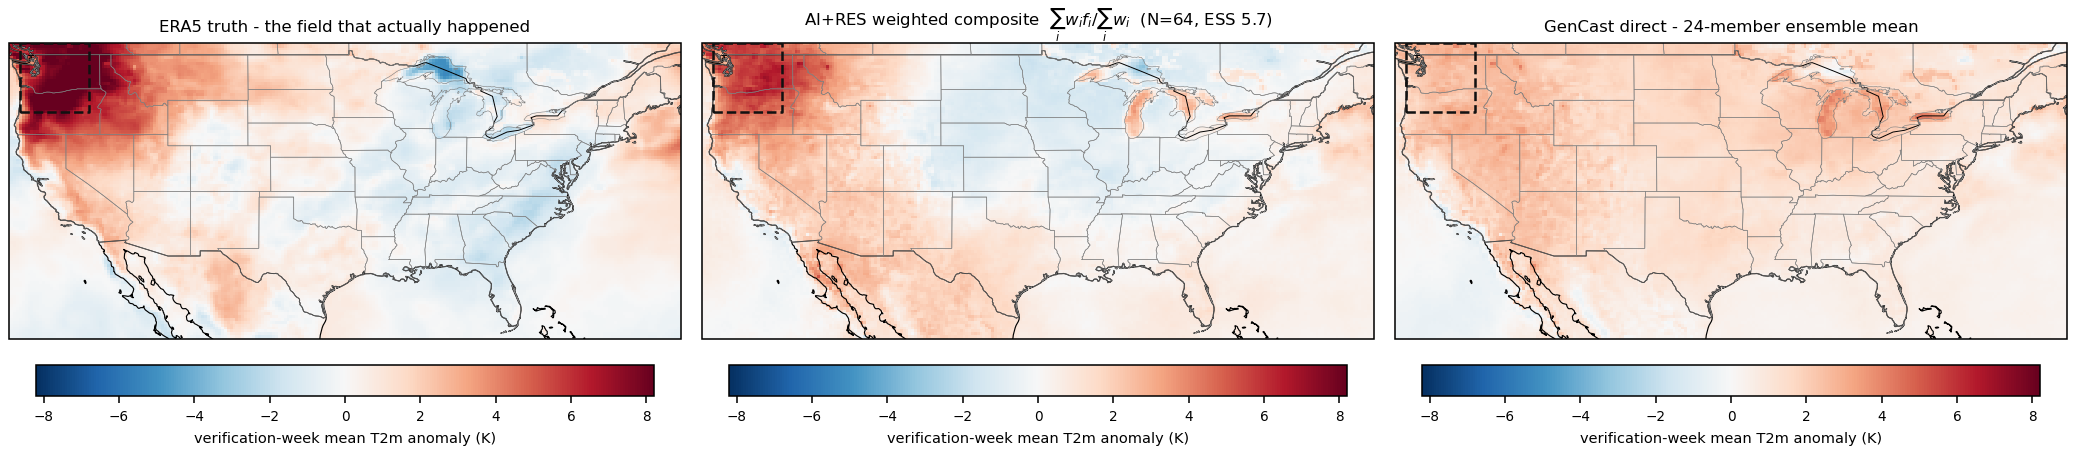
\includegraphics[width=\textwidth]{figs/pnw_anom_maps.png}
\caption{The 2021 Pacific Northwest heat dome, as maps of the week-average temperature anomaly.
\textbf{Left:} what happened. \textbf{Middle:} the AI+RES population three weeks out -- the dome
is in the right place with the right intensity. \textbf{Right:} the standard 24-member ensemble
average from the same starting point, which contains no dome at all. Dashed box is the scored
region. The middle panel is a weighted composite of trajectories selected for this event, so it
is a picture of where the method put its samples, not a forecast in the ordinary sense.}
\end{figure}

\begin{figure}[t]
\centering
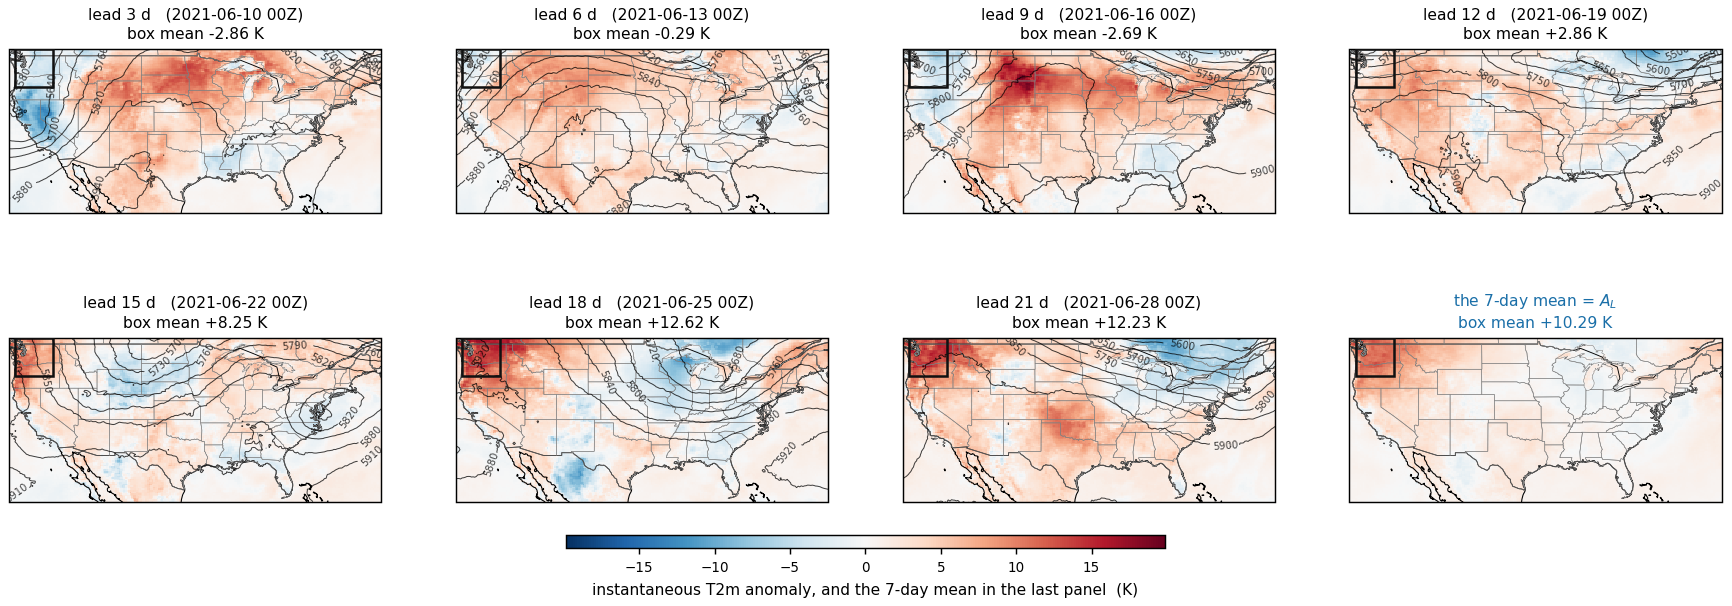
\includegraphics[width=\textwidth]{figs/pnw_map_walk.png}
\caption{Why the AI score is the ingredient. This is the single hottest surviving trajectory,
followed from the 3-day checkpoint to the event. At the 9-day checkpoint it had the
\emph{fourth-coolest} surface temperature of the 64 trajectories alive and would have been near
the bottom of any ``how hot is it now'' ranking. The scoring model ranked it tenth and gave it
the maximum eleven clones, because the upper-atmosphere ridge (contours) that later drives the
heat dome was already building offshore while the surface beneath it had not yet warmed.}
\end{figure}

\section*{5. What this is, and what it is not}

\textbf{It is} a demonstration, on nine out-of-sample cases, that concentrating a fixed compute
budget on the trajectories heading toward an extreme produces forecast members on events that
conventional sampling misses entirely at the same or larger budget, at a measured \$155 and 8
hours per forecast.

\textbf{It is not} a calibrated probability service. Three limits, stated plainly:

\begin{enumerate}
\item \textbf{Nine events cannot establish a hit rate.} The 6-of-7 figure has a wide interval
  around it. A 42-case hindcast campaign designed to produce a proper reliability curve is built
  and staged; it has not been run.
\item \textbf{The probabilities carry about a factor of two.} They are internally consistent --
  where plain sampling can resolve a probability at all, our estimate agrees with it -- but the
  absolute level at 64 trajectories is noisy, and the method gives no probability at all for an
  event milder than the population it has already concentrated.
\item \textbf{It samples the AI model's forecast distribution, not the atmosphere's.} The claim
  supported is that the method reaches the extreme tail of a state-of-the-art forecast model
  efficiently. Whether that model's tail is itself unbiased against the real climate is a
  separate question this work does not settle.
\end{enumerate}

\textbf{Next.} The 42-case calibration campaign, at an estimated \$1,700 of GPU time for its
first 12-case tier; a scoring function for hurricanes, where the weekly regional average used
here washes out a one-day landfall and a different target is needed; and lighter model pairs,
since the current pair requires an 80\,GB GPU per trajectory and a smaller one would cut the
per-forecast cost directly.

\end{document}
